\subsection{Confirmation on fresh questions}
\label{sec:exposure_confirmation}
The confirmation protocol reserves 128 new HC3 question identities, excludes the 1,712 retained questions and all 96 initial development/calibration identities, and splits generation into two disjoint 64-question shards. The shards share 64 separate public calibration identities. They use the same frozen watermark key and six source-blocked clients: direct resampling, reference smoothing and surrogate-ratio reweighting under each probability interface. Every client produces three attempts per source before quality-only selection and owner evaluation. The 2,304 attempts are retained. This cohort was fixed before the ratio development result and contains no support-pruning treatment.

\begin{figure}[ht]\centering
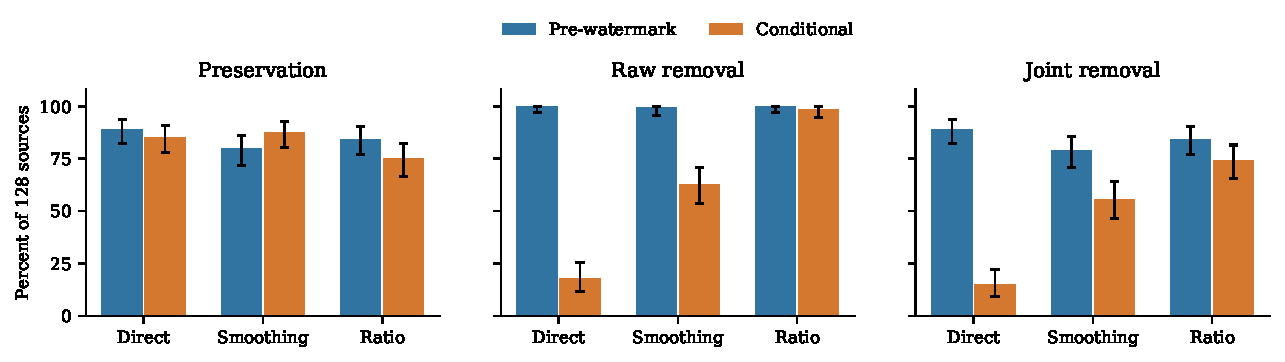
\includegraphics[width=\linewidth]{figures/exposure-confirmation.pdf}
\caption{Fresh-source TextSeal 2 confirmation on Qwen3.5-4B instruct: 128 HC3 answers, one frozen key, all sources detected at $p\leq0.001$. Each group names the probability-only client (direct resampling, confidence smoothing or reference-ratio reweighting); colors distinguish pre-watermark from estimated key-conditional probability exposure. Panels report preservation, owner non-detection and their joint event, each over all 128 sources after quality-only selection among three attempts. The auxiliary reference is Qwen3.5-0.8B. Error bars are exact binomial 95\% intervals conditional on these models and key; joint removal alone cannot separate retained signal from quality attrition.}
\label{fig:exposure-confirmation}
\end{figure}
\begin{table}[ht]\centering\small
\begin{tabular}{lrrrr}\toprule
Interface / client & Preserved & Raw removed & Joint removed & Joint 95\% CI\\\midrule
Pre / direct & 114/128 & 128/128 & 114/128 & [82.3, 93.9]\%\\
Pre / smooth & 102/128 & 127/128 & 101/128 & [70.8, 85.6]\%\\
Conditional / direct & 109/128 & 23/128 & 19/128 & [9.2, 22.2]\%\\
Conditional / smooth & 112/128 & 80/128 & 71/128 & [46.4, 64.3]\%\\
Pre / ratio & 108/128 & 128/128 & 108/128 & [76.9, 90.2]\%\\
Conditional / ratio & 96/128 & 126/128 & 95/128 & [65.7, 81.5]\%\\
\bottomrule\end{tabular}
\caption{Fresh 128-source, single-key confirmation after blind first-quality-passing selection from three attempts. Initially detected sources form the removal denominator. Intervals are exact binomial intervals, conditional on the evaluated key and models; paired differences are reported separately.}\end{table}


All 128 originals are detected. Figure~\ref{fig:exposure-confirmation} compares preservation, raw removal and joint removal for each client. Under direct resampling, changing exposure reduces joint removal from 114/128 to 19/128, while preservation passes change from 114/128 to 109/128. The paired difference is $-74.2$ percentage points, with a descriptive 95\% paired prompt-bootstrap interval $[-82.0,-65.6]$. Under smoothing, joint removal decreases from 101/128 to 71/128, with a paired difference of $-23.4$ points and interval $[-32.8,-14.1]$. These results confirm a restricted-client benefit on fresh questions.

The adaptive client changes the interpretation. Ratio reweighting removes 128/128 watermarks under pre-watermark exposure and 126/128 under conditional exposure. The latter preserves 96/128 outputs, of which 95 evade detection. Its 95/128 joint successes therefore reflect only one detected quality-preserving rewrite. The paired joint difference against pre-watermark exposure is $-10.2$ points, with interval $[-18.0,-2.3]$, but quality attrition explains most of that gap. A statistically distinguishable joint-success difference is not equivalent to robust watermark retention.

The intervals resample paired prompt identities 10,000 times with a fixed analysis seed. They are descriptive post-hoc uncertainty summaries, not prespecified multiple-comparison tests or uncertainty over training seeds and keys. The pooled human-null diagnostic is 0/128 at the native nominal threshold $0.001$; this small single-key set cannot validate a $0.1\%$ fixed-key false-positive rate precisely. No selected rewrite is a normalized word copy. Token-context overlap, source-blocking fallback counts and both shard-level tables remain in the analysis receipts.
